\documentclass[english]{eqconf}
\usepackage[T1]{fontenc}
\usepackage[utf8]{inputenc}
%\usepackage{showframe}
\usepackage{babel}
\usepackage{blindtext}
\usepackage{wrapfig}


\title{BİLDİRİ BAŞLIĞI}
\author{\authorspec{1}{Mücahit Bekin} ve
		\authorspec{*}{Barış Erkuş}%
}

\date{%
	\affils{1}{Prof. Dr., İnşaat Müh. Bölümü, Abece Üniversitesi, Güzelkent}\\
	\affils{*}{Araş. Gör., Jeofizik Müh. Bölümü, Abece Teknik Üniversitesi, Büyükkent}\\
	\email{gönderenyazar@kurum}%
}

 
\begin{document}

%%% Keep thes lines
\fixturkishbug
\maketitle
\thispagestyle{firststyle}
%%%%%%%

 
%%% A Turkish Abstract has to be provided if the paper is in Turkish
\begin{ozet}
\blindtext
\end{ozet}

\begin{anahtarkelimeler}
anahtar kelime1, anahtar kelime2, anahtar kelime3.
\end{anahtarkelimeler}


%%% All papers (both Turkish and English) have to provide English abstract
\begin{abstract} 
\blindtext
\end{abstract}

\begin{keywords}
keyword1, keyword2, keyword3.
\end{keywords}



 
\section{INTRODUCTION}
The Monty Hall problem...
$x=\frac{a}{b}$
 
\subsection{Theory}

\blindtext

\section{INTRODUCTION}

\blindtext

\subsubsection*{Theory}

\blindtext

\blindtext
\begin{wrapfigure}{r}{0.4\textwidth}
	\vspace{-12pt}
	\centering
	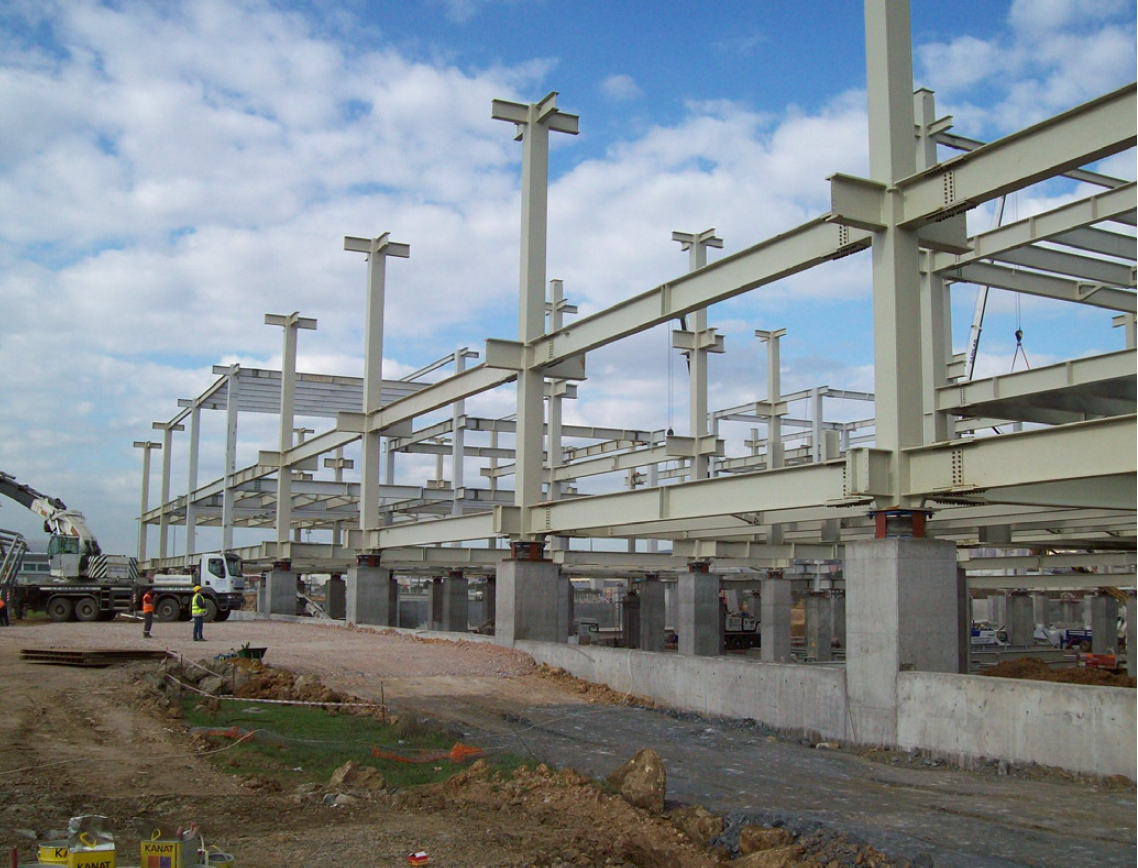
\includegraphics[scale=0.2]{b.PNG}
	\caption{A boat.}
	\label{fig:boat1}
	\vspace{-10pt}
\end{wrapfigure}
\blindtext

\blindtext

\blindtext


\begin{figure}[]
	\centering
	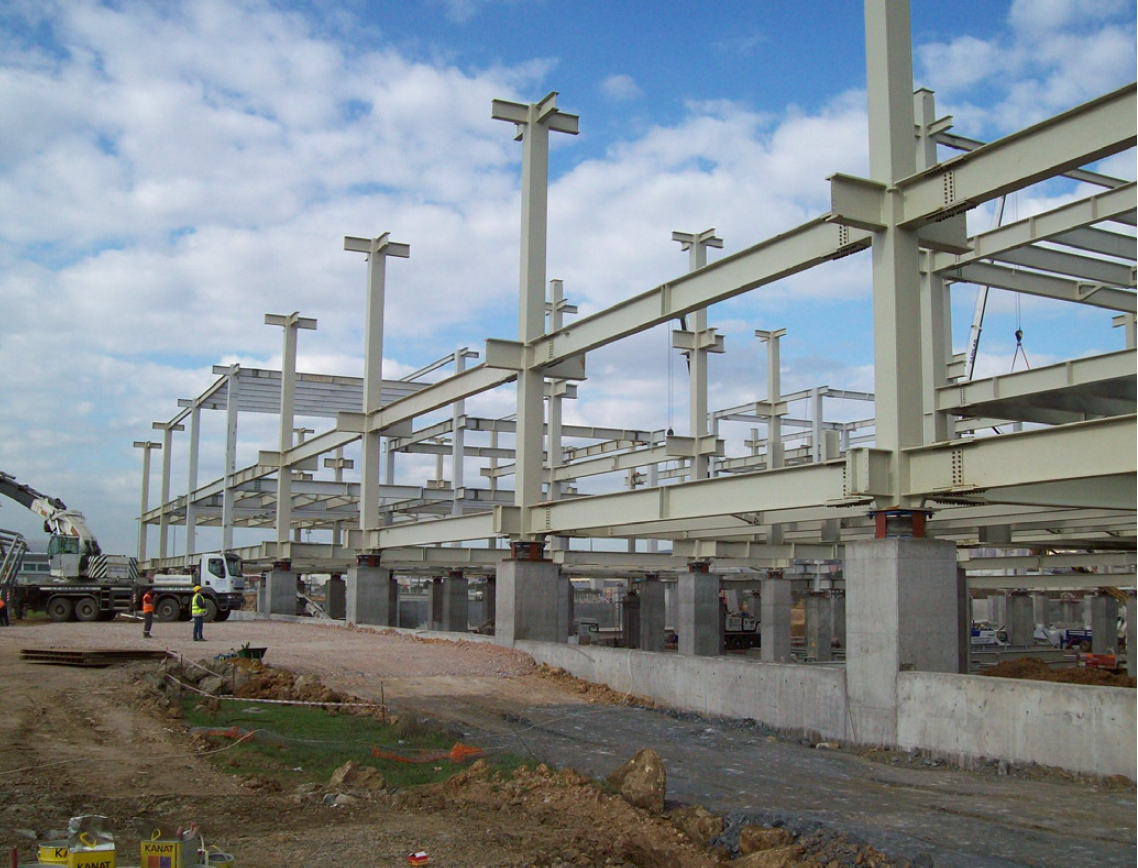
\includegraphics[scale=0.4]{b.PNG}
	\caption{A boat.}
	\label{fig:boat1}
\end{figure}


\blindtext

\blindtext

\blindtext

\blindtext

\blindtext \blindtext \blindtext \blindtext

\begin{table}[]
	\setlength\abovecaptionskip{0pt}
	\setlength\belowcaptionskip{15pt}
	\centering
		\caption{Your first table.}
		\label{tab:table1}
		\begin{tabular}{l|c|r} % <-- Alignments: 1st column left, 2nd middle and 3rd right, with vertical lines in between
			\textbf{Value 1} & \textbf{Value 2} & \textbf{Value 3}\\
			$\alpha$ & $\beta$ & $\gamma$ \\
			\hline
			1 & 1110.1 & a\\
			2 & 10.1 & b\\
			3 & 23.113231 & c\\
		\end{tabular}
\end{table}

\blindtext

\blindtext

\begin{wraptable}{l}{6cm}
	\setlength\abovecaptionskip{0pt}
	\setlength\belowcaptionskip{15pt}
	\vspace{-12pt}
	\centering
	\caption{Your first table.}
	\label{tab:table1}
	\begin{tabular}{l|c|r} % <-- Alignments: 1st column left, 2nd middle and 3rd right, with vertical lines in between
		\textbf{Value 1} & \textbf{Value 2} & \textbf{Value 3}\\
		$\alpha$ & $\beta$ & $\gamma$ \\
		\hline
		1 & 1110.1 & a\\
		2 & 10.1 & b\\
		3 & 23.113231 & c\\
	\end{tabular}
\end{wraptable}

\blindtext

\blindtext

\begin{figure}[h]
	\centering
	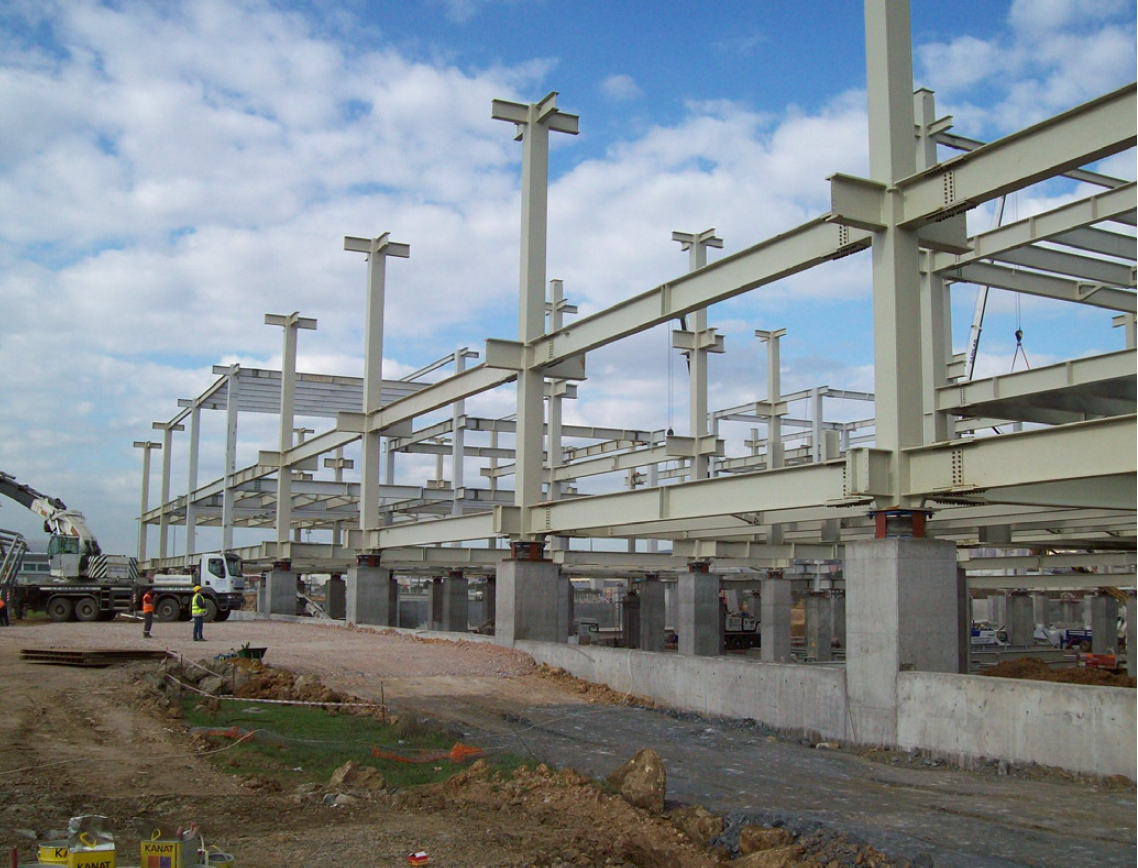
\includegraphics[scale=0.4]{b.PNG}
	\caption{A boat.}
	\label{fig:boat1}
\end{figure}

\blindtext

\blindtext



\end{document}